\chapter{Introduction}
\label{chap:intro}

\textbf{Software architecture} is a field of studies that allows one to understand software as components or modules and relationships between these components. Architectural drawings can be used to understand software, to communicate about the software in the software teams and with stakeholders. 
Horizontal layering and vertical layering has been applied several times to finegrain the questions and details to software. Horizontal layout is characterized with stack based view growing in y axis, while verticaly layered architecture explains the relations of distributed systems in x axis.
For example, horizontal layered architecture that is used in OSI model, depicted below explains how data is packed and unpacked and routed across computer systems in a network. 
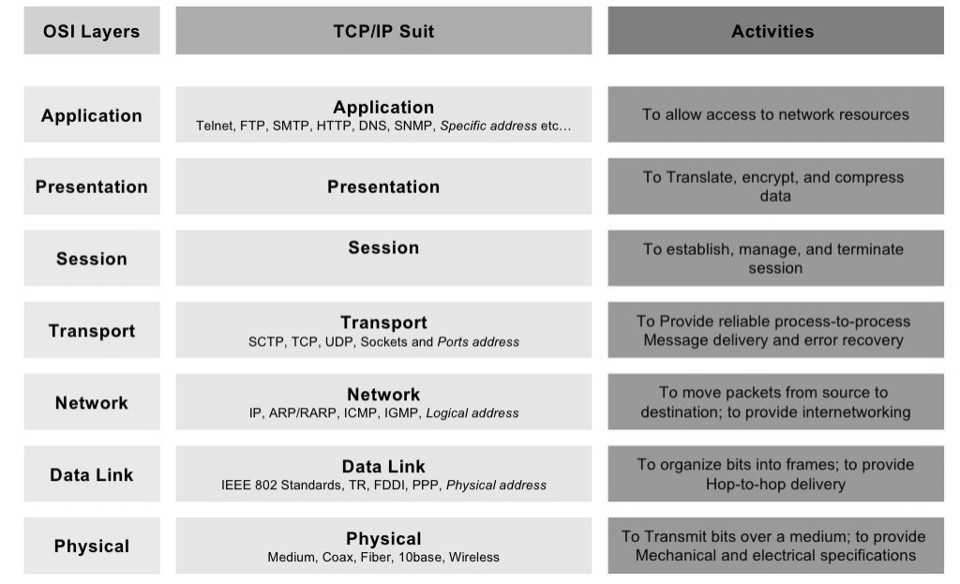
\includegraphics[scale=0.5]{osi.png}\\[\fill] 

While, vertical layering can explain the deployment view of distributed systems. Those layering views are staring points for understanding a software development task at hand. 
For example, for a software developer who is working on a concrete JIRA task that states a problem as follows: Given a desktop client UI for medicine management, extend the menu with a new functionality "Dose" that updates the backend application class "MedicineService" and its respective database table "Medicine".A scenario like that is called a \textbf{functional requirement}. For such case an architectural sketch as depicted below would suffice for an initial kick off meeting. The drawing splits a product into deployment components each residing on its own server, when deployed at customer. The drawing also illustrates frameworks, libraries and languages used. Functional requirements can be proved for correctness by manual tests of some usage scenario.

  %\includegraphics[width=4cm]{ClientServer.gif}\\[\fill]
  
  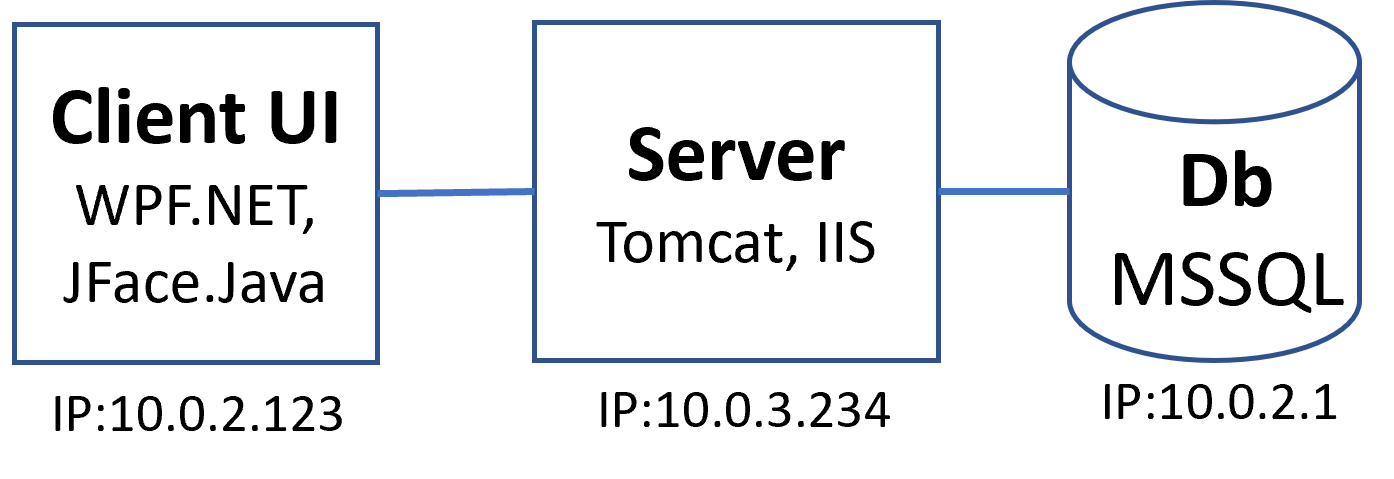
\includegraphics[scale=0.5]{client-server.png}\\[\fill] 

Having got these notations for describing software applications one may ask questions about software qualities, known as \textbf{quality requirements} regarding the performance of the backends service ability of fetching the data from the database. Does the server fetch the DB tables optimally or how is the query performance?, Does it cache the intermediate objects ? Does it use DTOs to access database objects or are string based SQL queries used for fetching the result set? What can we say about securing the data in the database, is data secure against SQL injections.
Quality requirements are much harder to achieve and prove. One type of proves for correct implementation are stress tests, performance tests and so on. 

 ~\citep{lazypropagation2010,ambiguity2010}. \lipsum[2-10]
